\subsection{UC1: Autenticazione}
\label{sec:UC1}
\begin{figure}[!ht]
    \caption{Diagramma di UC1: Autenticazione}
    \vspace{10px}
    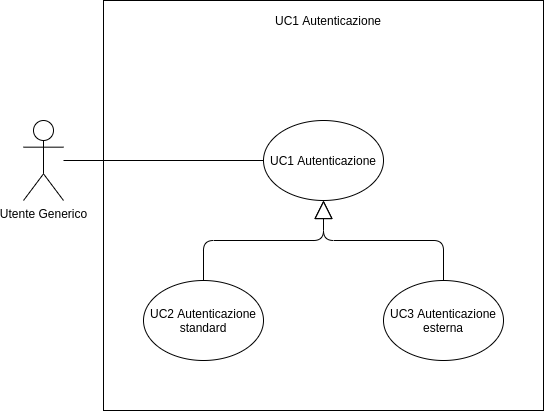
\includegraphics[scale=0.5]{../../../Images/AnalisiRequisiti/UC01}
    \centering
\end{figure}
\begin{itemize}
    \item \textbf{Descrizione:} permette l'autenticazione di un utente;
    \item \textbf{Attore Primario:} utente non autenticato;
    \item \textbf{Attore Secondario:} servizio di autenticazione esterno;
    \item \textbf{Precondizione:} l'utente non si è ancora autenticato;
    \item \textbf{Input:} pressione bottone \textit{login};
    \item \textbf{Postcondizione:} l'utente è autenticato;
    \item \textbf{Scenario Principale:}
          \begin{itemize}
              \item l'utente entra nella pagina;
              \item preme il bottone per il login;
              \item viene indirizzato alla pagina di login fornita dal servizio di autenticazione.
          \end{itemize}
\end{itemize}
\newpage